\section{Hall effect}
A popular choice to gather information about charge carrier density and mobility
is a Hall effect experiment. 
This section introduces the theoretical background of the Hall effect 
by summarizing \citeauthoryear{grundmann}, chapter 15.2.1.

\begin{figure}
	\centering
	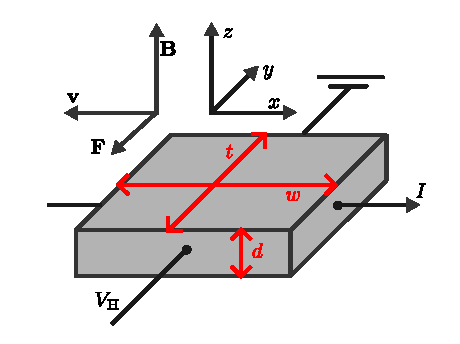
\includegraphics{../assets/hall_geometry.pdf}
	\caption{Schematic structure for Hall effect measurements.
		\imcitetwo{grundmann}}
	\label{fig:hall}
\end{figure}
The geometrical arrangement required for Hall effect measurements
is displayed in \cref{fig:hall}.
A magnetic field $\mathbf{B}=B_z \cdot \hat{z}$ penetrates
a semiconductor sample.
A current density $\mathbf{j}$ is induced along the $x$-direction inside the sample 
as a response to an external electric field $\mathbf{E}=E_x \cdot \hat{x}$.
Due to the magnetic force, electrons are deflected and a current in
$y$-direction establishes until the resulting electric force in $y$-direction
fully compensates the magnetic force.
The system equilibrates for $\mathbf{j} = j_x \cdot \hat{x}$.

To describe the system in detail for one majority charge carrier, one can use the 
equation of motion from relaxation time approximation:
\begin{equation}
	m^{*} \frac{\mathbf{v}}{\tau}=q(\mathbf{E}
	+\mathbf{v}\times \mathbf{B}).
\end{equation}
In this equation, $m^{*}$ is the effective mass of the charge carrier, $q$ is the charge, 
$\mathbf{v}$ the average electron velocity and $\tau$ the relaxation time constant.
With $\mathbf{j}=nq\mathbf{v}$ and the resistivity tensor $\hat{\rho}$, 
this vector equation can be brought into a linear transformation of the form
$\mathbf{E}=\hat{\rho}\mathbf{j}$ or more explicit:
\begin{equation}
	\label{eq:mej}
	\begin{pmatrix}
		E_{x} \\
		E_{y} \\
		E_{z}
	\end{pmatrix}
	=
	\begin{pmatrix}
		\frac{m^{*}}{\tau nq^{2}} & - \frac{B_{z}}{nq}        & 0                         \\
		\frac{B_{z}}{nq}          & \frac{m^{*}}{\tau nq^{2}} & 0                         \\
		0                         & 0                         & \frac{m^{*}}{\tau nq^{2}}
	\end{pmatrix}
	\begin{pmatrix}
		j_{x} \\
		j_{y} \\
		j_{z}
	\end{pmatrix}.
\end{equation}
The system equilibrates for $\mathbf{j} = j_x \cdot \hat{x}$ and with \cref{eq:mej}, the following
relationship holds true: $E_{y} = B_{z} / (nq) j_{x}$.
Since $E_y$, $j_x$ and $B_z$ are directly measurable quantities,
they are used to define the Hall coefficient $R_{\mathrm{H}}$.
This directly relates the Hall coefficient to the carrier density $n$:
\begin{align}
	R_{\mathrm{H}}&=\frac{E_{y}}{j_{x}B_{z}}=\frac{1}{nq},
	\label{eq:hall_coefficient} \\
	n&=\frac{j_{x}B_{z}}{E_{y}q} = \frac{1}{R_{\mathrm{H}}q}.
	\label{eq:hall_concentration}
\end{align}

By using \cref{eq:mej} without additional substitutions and the mobility tensor 
$\hat{\mu}$, a linear transformation $\mathbf{E}=\hat{\mu} \mathbf{v}$ 
can be established:
\begin{equation}
	\begin{pmatrix}
		E_{x} \\
		E_{y} \\
		E_{z}
	\end{pmatrix}
	=\begin{pmatrix}
		\mu_\mathrm{H}^{-1} & -B_{z}              & 0                   \\
		B_{z}               & \mu_\mathrm{H}^{-1} & 0                   \\
		0                   & 0                   & \mu_\mathrm{H}^{-1}
	\end{pmatrix}
	\begin{pmatrix}
		v_{x} \\
		v_{y} \\
		v_{z}
	\end{pmatrix}.
	\label{eq:mev}
\end{equation}
The hall mobility in \cref{eq:mev} is defined as $\mu_{\mathrm{H}}= q\tau / m^{*}$.
Applying the equilibrium condition $\mathbf{v}=v_x \cdot \hat{x}$ and evaluating 
\cref{eq:mev} component-wise yields $v_{x} = \mu_{\mathrm{H}}E_{x}$ and 
$E_{y}=B_{z}v_{x}=B_{z}\mu_{\mathrm{H}}E_{x}$.
Using \cref{eq:hall_coefficient} and the sample's resistivity $\rho=E_x / j_x$, 
the hall mobility can be expressed as:
\begin{equation}
	\mu_{\mathrm{H}}=\frac{E_y}{B_z E_x} =\frac{R_{\mathrm{H}}}{\rho} =\frac{1}{nq\rho}.
	\label{eq:hall_mobility}
\end{equation}

\subsection{Van der Pauw Method}
\begin{figure}
	\centering
	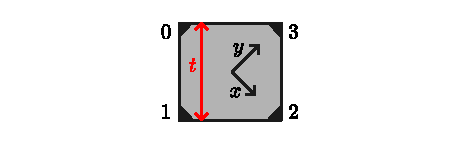
\includegraphics{../assets/van_der_pauw.pdf}
	\caption{Van der Pauw sample edges.}
	\label{fig:van_der_pauw}
\end{figure}

The Van der Pauw Method is a measurement technique to measure the resistivity as well 
as the hall coefficient.
It is possible to measure samples with nearly arbitrary flat shapes and examine its 
resistivity, mobility as well as it's carrier density. 
The derivations in this section follow \citeauthoryear{van_der_pauw}.

Only samples that met the subsequent conditions can be measured with the Van der Pauw 
method:
\begin{itemize}
	\item The contacts are at the circumference of the sample.
	\item The contacts are sufficiently small (compared to the sample size).
	\item The sample is homogeneous and isotropic cocerning doping as well as thickness.
	\item The surface of the sampele is singly connected, i.e., the sample does not
	have isolated holes.
\end{itemize}
To utilize the Van der Pauw method, four ohmic contacts need to be attached to the 
sample.
These contacts should be as small as possible and as close as possible to the sample's 
periphery. 
All contacts and all wires should be constructed from the same material. 

A Van der Pauw experiment starts with measurement of the resistivity $\rho$.
The four contacts on the sample are numbered from \num{0} to \num{3} in a 
counterclockwise manner as shown in \cref{fig:van_der_pauw}. 
To systemize the measurement, these contact labels can be identified with the 
elements of the residue class ring $\mathbb{Z}/4\mathbb{Z}$ (i.e. $3+2=\mod(5,4)=1$).
Let $i$ be an arbitrary element of $\mathbb{Z}/4\mathbb{Z}$.
The current $I_{i, i+1}$ is defined as the positive current injected into contact $i$ 
and extracted from contact $i+1$.
The voltage $V_{i, i+1}$ is given by the potential difference between contact $i$ and 
$i+1$ as $V_{i, i+1}=V_{i+1}-V_i$. 
With these definitions, the resistivity can be calculated as 
$R_{i, i+1; i+2, i+3}=V_{i+2, i+3} / {I_{i, i+1}}$. 
Van der Pauw's theorem states that the resistivity can be calculated using 
$r_1=R_{i, i+1; i+2, i+3}$ and $r_2=R_{i+1, i+2; i+3, i+4}$ as the two independent 
resistances:
\begin{align}
	\rho=\frac{\pi d}{\ln(2)} \left( \frac{r_1+r_2}{2} \right)f
	\left( \frac{r_1}{r_2} \right), \label{eq:hall_resistivity}\\
	\frac{r_1-r_2}{r_1+r_2}=f \cosh^{-1} \left( \frac{\exp(\ln(2 /f))}{2} \right),
	\label{eq:hall_resistivity_f}
\end{align}
where $d$ is the thickness of the sample and $f$ is a correction factor that satisfies 
\cref{eq:hall_resistivity_f}. 
The reciprocal theorem states that the resistances obey the relation 
$R_{i, i+1; i+2, i+3}=R_{i+2, i+3; i, i+1}$ and 
$R_{i, i+1;i+2, i+3}=R_{i+1, i; i+3, i+2}$.
Therefore, the resistivity can be measured with four different contact configurations to
increase measurement accuracy.

Within the Van der Pauw configuration and the geometry depicted in 
\cref{fig:van_der_pauw}, it is also possible to determine the Hall 
coefficient $R_{\mathrm{H}}$ if a homogeneous magnetic field perpendicular to the 
samples surface is applied.
Since $I_{i, i+2}= j_x A$ for a cross-sectional area 
$A = \sqrt{2} d t$ and the Hall voltage $V_{i+1, i+3} = E_y \sqrt{2} t$,
the Hall coefficient can be calculated using \cref{eq:hall_coefficient}:
\begin{equation}
	R_{\mathrm{H}}=\frac{d}{I_{i, i+2}B_{z}} 
	[V_{i+1, i+3}(B_{z}=0)-V_{i+1, i+3}(B_{z}>0)].
	\label{eq:hall_coefficient_van_der_pauw}
\end{equation}
The difference term in  \cref{eq:hall_coefficient} accounts for the Hall voltage that 
originates from the earths magnetic field.

\subsection{Notational Conventions}
In \cref{eq:hall_coefficient_van_der_pauw}, the thickness $d$ is
not measured as part of the experiment, but is given as a constant and was measured
beforehand. 
Therefore, the Hall-Experiment itself does not yield thickness information.
To represent this via notation, thickness independent (sheet) quantities are defined and 
denoted with '$\square$' as a subindex.
For reference, $R_{\mathrm{H} \square}=R_\mathrm{H} / d$ is defined as the sheet 
Hall-coefficient, $n_\square = n d = 1 / (R_\mathrm{H \square}q)$ is the sheet carrier 
concentration. 
Since $\mu_\mathrm{H}$ is independent of the thickness, 
it is not denoted with a subindex.

\begin{figure*}
	\centering
	\begin{subfigure}{0.45\linewidth}
			\centering
			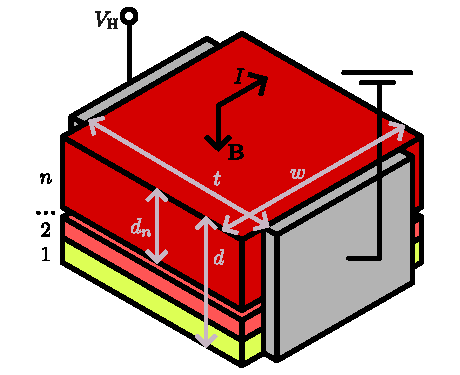
\includegraphics[width=\linewidth]{../assets/multilayer_hall_1.pdf}
			\caption{Geometric arrangement.}
			\label{fig:multilayer_hall_1}
		\end{subfigure}
		\begin{subfigure}{0.45\linewidth}
			\centering
			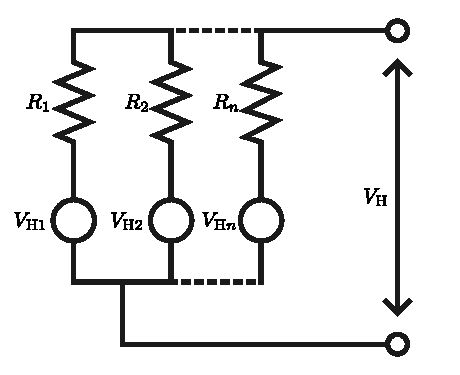
\includegraphics[width=\linewidth]{../assets/multilayer_hall_2.pdf}
			\caption{Equivalent circuit.}
			\label{fig:multilayer_hall_2}
		\end{subfigure}
	\caption{Schematic representation of the Hall effect in multilayer samples. 
	\imcitetwo{multilayer}}
	\label{fig:multilayer_hall}
\end{figure*}

\subsection{ Multilayer Hall Analysis}
This section follows \citeauthoryear{multilayer}.
For multilayer samples, Hall effect data analysis complicates due to the different
contributions of each layer.
As depicted in \cref{fig:multilayer_hall_1}, each layer $i$ with a specific thickness 
$d_i$ and conductivity $\sigma_i$ carries a current $I_{xi}$ in $x$-direction.
Since the layers are connected in parallel, the total current is 
given by Kirchhoff's current law:
\begin{equation}
	I_x = \sum_i I_{xi}.
\end{equation}
Using Ohm's law and $I_x=j_x A$, where $A=t d = t \sum_i d_i$ is the cross-sectional area of 
the sample perpendicular to the $x$-direction, a condition for the total Hall sheet 
conductivity $\sigma_\mathrm{\square H}$ can be derived:
\begin{align}
	I_{x}&=j_{x}dt=\sigma E_{x} dt \notag\\
	&=\sum_{i}I_{x i}=\sum_{i}j_{x i} d_{i}t \notag\\
	&=\sum_{i}\sigma_{i} E_{x}d_{i}t, \\
	\sigma d&=\sum_{i}\sigma_{i}d_{i}, \\
	\sigma_{\mathrm{\square}}&=\sum_{i} \sigma_{\square i}.
	\label{eq:multilayer_sum_1}
\end{align}

Using the equivalent circuit diagram in \cref{fig:multilayer_hall_2} and the conductance
$G_i = R_i^{-1}$, an expression for the Hall voltage $V_{\mathrm{H}}$ is found:
\begin{equation}
	V_{\mathrm{H}}=\frac{\sum_{i}V_{\mathrm{H}i}G_{i}}{\sum_{i}G_{i}}.
	\label{eq:multilayer_hall_voltage}
\end{equation}
The conductance depends on to the conductivity and the geometrical arrangement of the 
sample as $G_i = \sigma_i d_i w/ t$. Substituting this into 
\cref{eq:multilayer_hall_voltage} yields:
\begin{equation}
	V_{\mathrm{H}}=\frac{\sum_{i}V_{\mathrm{H}i}  
	\sigma_{i}d_{i}}{\sum_{i} \sigma_{i}d_{i}}.
	\label{eq:multilayer_hall_voltage_2}
\end{equation}
Using \cref{eq:mej}, $E_y t = V$ and $I_x=j_x d t$, one finds an expression 
for the Hall voltage:
\begin{align}
	E_{y}&=R_{\mathrm{H}}j_{x}B_{z},\\
	\frac{V_{\mathrm{H}}}{t}&=R_{\mathrm{H}}\frac{I_{x}}{t d}B_{z}.
	\label{eq:multilayer_hall_r}
\end{align}
\Cref{eq:multilayer_hall_r} is valid for each layer with corresponding current density
$j_{xi}$, hall voltage $V_{\mathrm{H}i}$ and thickness $d_i$ as well as for the total 
system:
\begin{align}
	V_{\mathrm{H}i} &= \frac{R_{\mathrm{H}i}I_{xi} B_z}{d_{i}}, \\
	V_{\mathrm{H}}&=\frac{R_{\mathrm{H}}I_{x}B_z}{d}.
	\label{eq:multilayer_hall_r_2}
\end{align}
Substituting \cref{eq:multilayer_hall_r_2} into \cref{eq:multilayer_hall_voltage_2} and
using the identity $I_{xi} /I=\sigma_{i}d_{i} /\sigma d$ results in:
\begin{align}
	\frac{R_{\mathrm{H}}}{d}=\frac{\sum R_{\mathrm{H}i} \sigma_{i}^{2} d_{i}}
	{(\sigma d)^2}, \\
	R_{\mathrm{H \square}}\sigma_{\square}^2=\sum_{i}R_{\mathrm{H}\square i} 
	\sigma_{\square i}^{2}.
	\label{eq:multilayer_sum_2}
\end{align}
\Cref{eq:multilayer_sum_1} and \cref{eq:multilayer_sum_2} are two main results of the 
multilayer Hall analysis and are sufficient to analyze the unusual \ce{ZnO} sample.